\documentclass[12pt, a4paper]{report}
\usepackage[top=1cm, left=1cm, right=1cm]{geometry}

\usepackage[utf8]{inputenc}
\usepackage[russian]{babel}

\usepackage{array}
\newcolumntype{M}[1]{>{\centering\arraybackslash}m{#1}}

\usepackage{hyperref}
\hypersetup{
	colorlinks,
	citecolor=black,
	filecolor=black,
	linkcolor=black,
	urlcolor=black
}

\usepackage{sectsty}
\allsectionsfont{\centering}

\usepackage{indentfirst}
\setlength\parindent{24pt}

\usepackage{algorithm}
\usepackage[noend]{algpseudocode}

\usepackage{listings}
\usepackage{xcolor}
\definecolor{codegreen}{rgb}{0,0.6,0}
\definecolor{codegray}{rgb}{0.5,0.5,0.5}
\definecolor{codepurple}{rgb}{0.58,0,0.82}
\definecolor{backcolour}{rgb}{0.95,0.95,0.92}
\lstdefinestyle{mystyle}{
    backgroundcolor=\color{backcolour},
    commentstyle=\color{codegreen},
    keywordstyle=\color{magenta},
    numberstyle=\normalsize\color{codegray},
    stringstyle=\color{codepurple},
    basicstyle=\ttfamily\footnotesize,
    breakatwhitespace=false,
    breaklines=true,
    captionpos=b,
    keepspaces=true,
    numbers=left,
    numbersep=5pt,
    showspaces=false,
    showstringspaces=false,
    showtabs=false,
    tabsize=2
}

\usepackage{graphicx}
\graphicspath{ {plots/pictures/}{assets/pictures} }

\begin{document}
	\begin{titlepage}
		\begin{center}
			\large \textbf{Министерство науки и высшего образования Российской Федерации} \\
			\large \textbf{Федеральное государственное бюджетное образовательное учреждение высшего образования} \\
			\large \textbf{«Российский химико-технологический университет имени Д.И. Менделеева»} \\

			\vspace*{4cm}
			\LARGE \textbf{ОТЧЕТ ПО ЛАБОРАТОРНОЙ РАБОТЕ №5}

			\vspace*{4cm}
			\begin{flushright}
				\Large
				\begin{tabular}{>{\raggedleft\arraybackslash}p{9cm} p{10cm}}
					Выполнил студент группы КС-36: & Золотухин А.А. \\
					Ссылка на репозиторий: & https://github.com/ \\
					& MUCTR-IKT-CPP/ \\
					& ZolotukhinAA\_36\_ALG \\
					Принял: & Крашенников Роман Сергеевич \\
					Дата сдачи: & 24.03.2025 \\
				\end{tabular}
			\end{flushright}

			\vspace*{6cm}
			\Large \textbf{Москва \\ 2025}
		\end{center}
	\end{titlepage}

	\tableofcontents
	\thispagestyle{empty}
	\newpage

	\pagenumbering{arabic}

	\section*{Описание задачи}
	\addcontentsline{toc}{section}{Описание задачи}
	\large
	\begin{enumerate}
		\item Создайте взвешенный граф, состоящий из [10, 20, 50, 100] вершин.
		\begin{itemize}
			\item каждая вершина графа связана со случайным количеством вершин, минимум с [3, 4, 10, 20];
			\item веса рёбер задаются случайным значением от 1 до 20;	
			\item каждая вершина графа должна быть доступна, т.е. до каждой вершины графа должен обязательно существовать путь до каждой вершины, необязательно прямой;
			\item (Можно использовать генератор из предыдущей лабораторной работы.)
		\end{itemize}
		\item Выведите получившийся граф в виде матрицы смежности.
		\item Для каждого графа требуется провести серию из 5-10 тестов, в зависимости от времени, затраченного на выполнение одного теста. Необходимо:
		\begin{itemize}
			\item найти кратчайшие пути между всеми вершинами графа и их длину с помощью алгоритма Флойда-Уоршелла.
		\end{itemize}
		\item В рамках каждого теста необходимо замерить потребовавшееся время на выполнение задания из пункта 3 для каждого набора вершин. По окончании всех тестов построить график, используя полученные замеры времени, где на ось абсцисс (X) нанести N - количество вершин, а на ось ординат (Y) - значения затраченного времени.
	\end{enumerate}

	\newpage

	\section*{Описание метода/модели}
	\addcontentsline{toc}{section}{Описание метода/модели}
	\large

	\newpage

	\section*{Выполнение задачи}
	\addcontentsline{toc}{section}{Выполнение задачи}

	\newpage
	\vfill

	\begin{figure}[h]
		\centering
		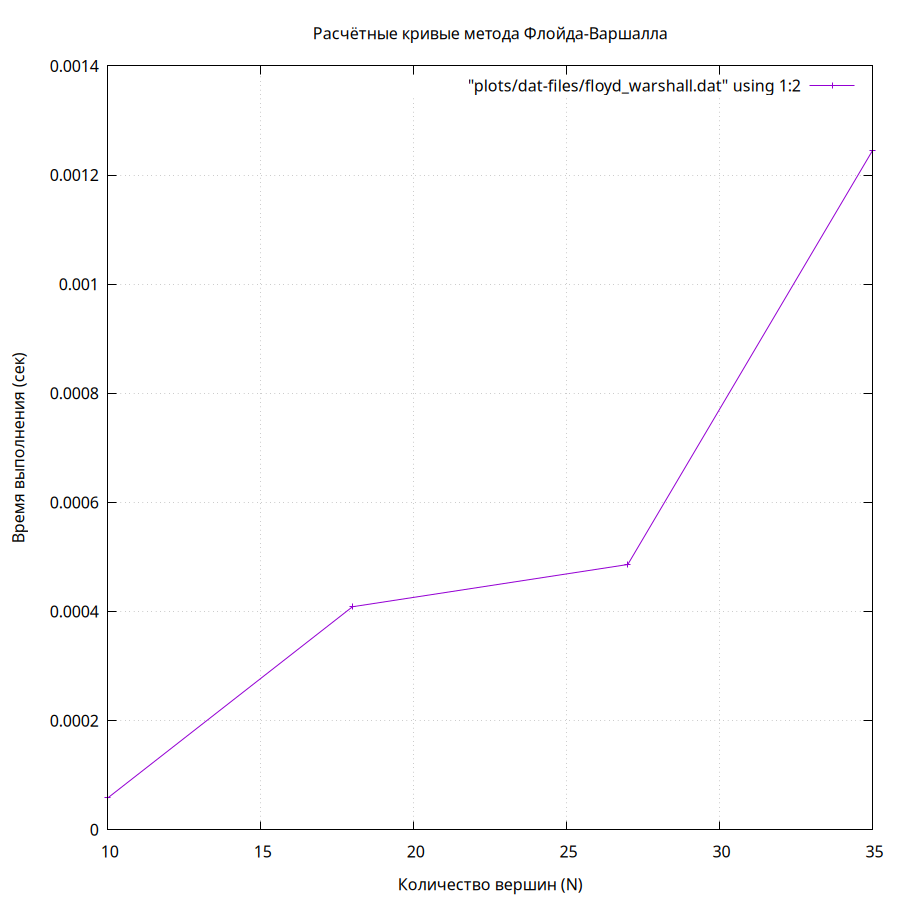
\includegraphics[width=300pt]{floyd_warshall.png}
		\caption{График.}
	\end{figure}

	\begin{figure}[h]
		\centering
		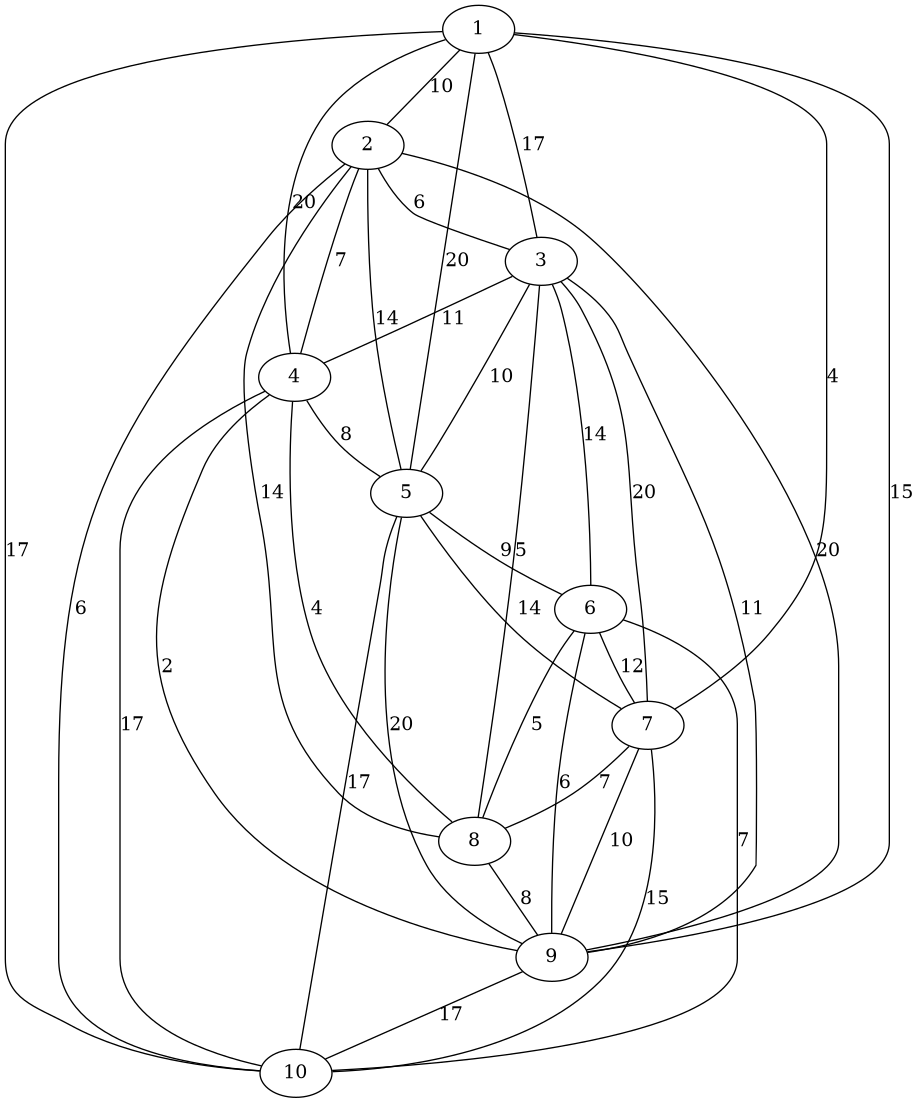
\includegraphics[width=300pt]{graph_size_10_1.png}
		\caption{Граф 1 с 10 вершинами.}
	\end{figure}
	\begin{figure}[h]
		\centering
		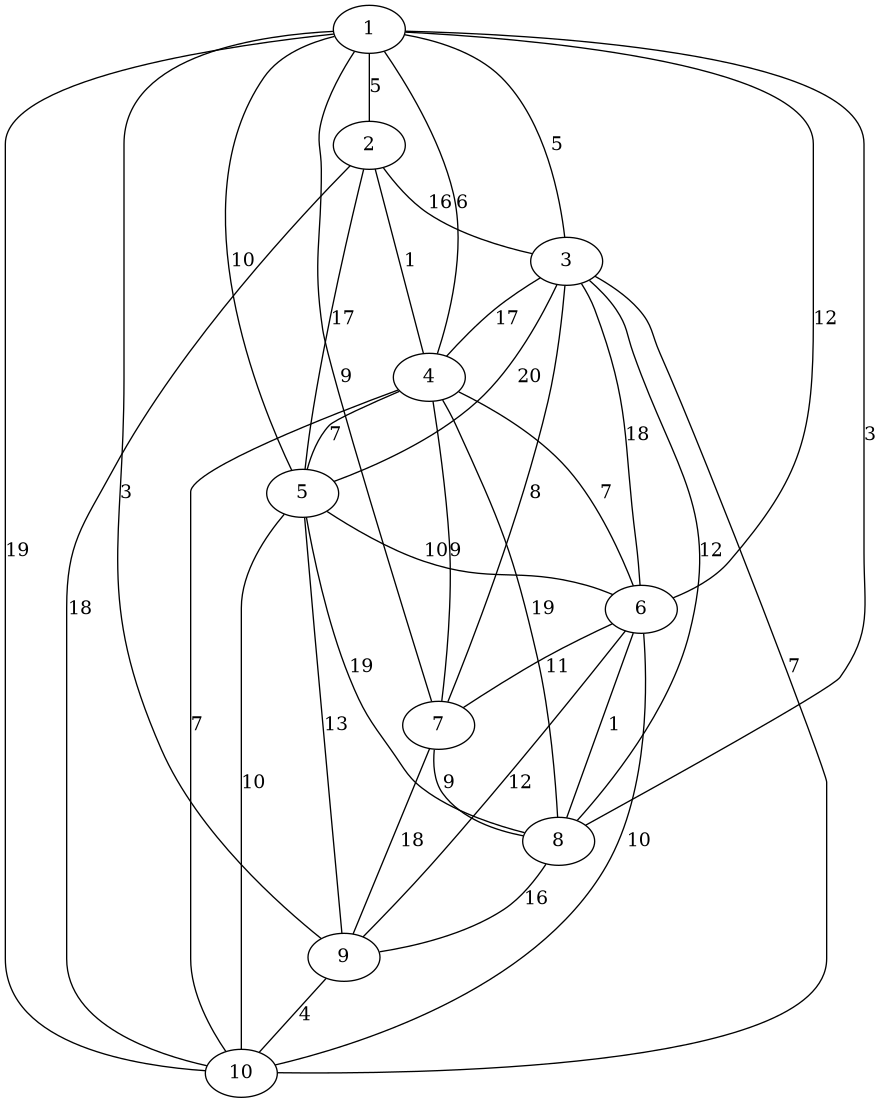
\includegraphics[width=300pt]{graph_size_10_2.png}
		\caption{Граф 2 с 10 вершинами.}
	\end{figure}
	\begin{figure}[h]
		\centering
		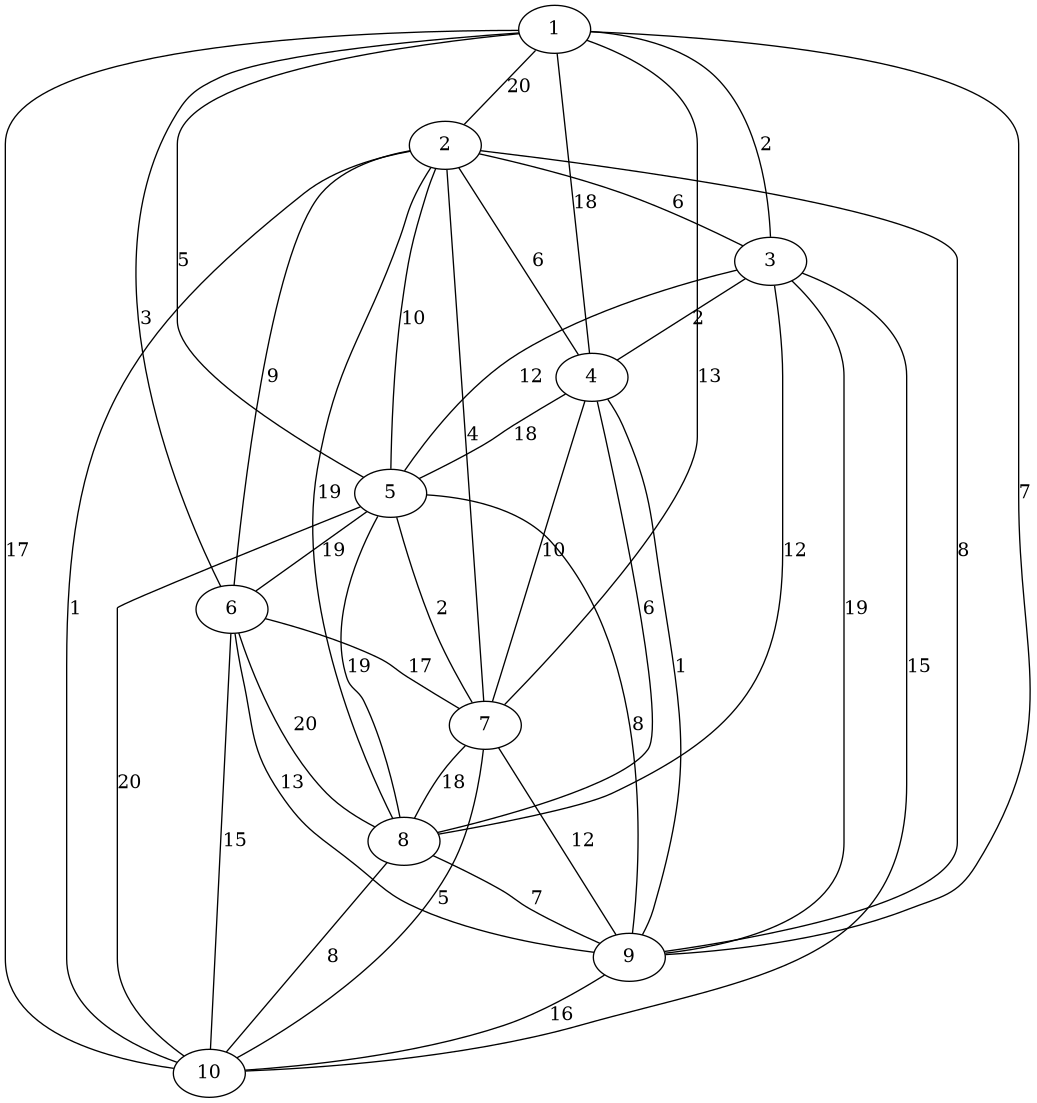
\includegraphics[width=300pt]{graph_size_10_3.png}
		\caption{Граф 3 с 10 вершинами.}
	\end{figure}
	\begin{figure}[h]
		\centering
		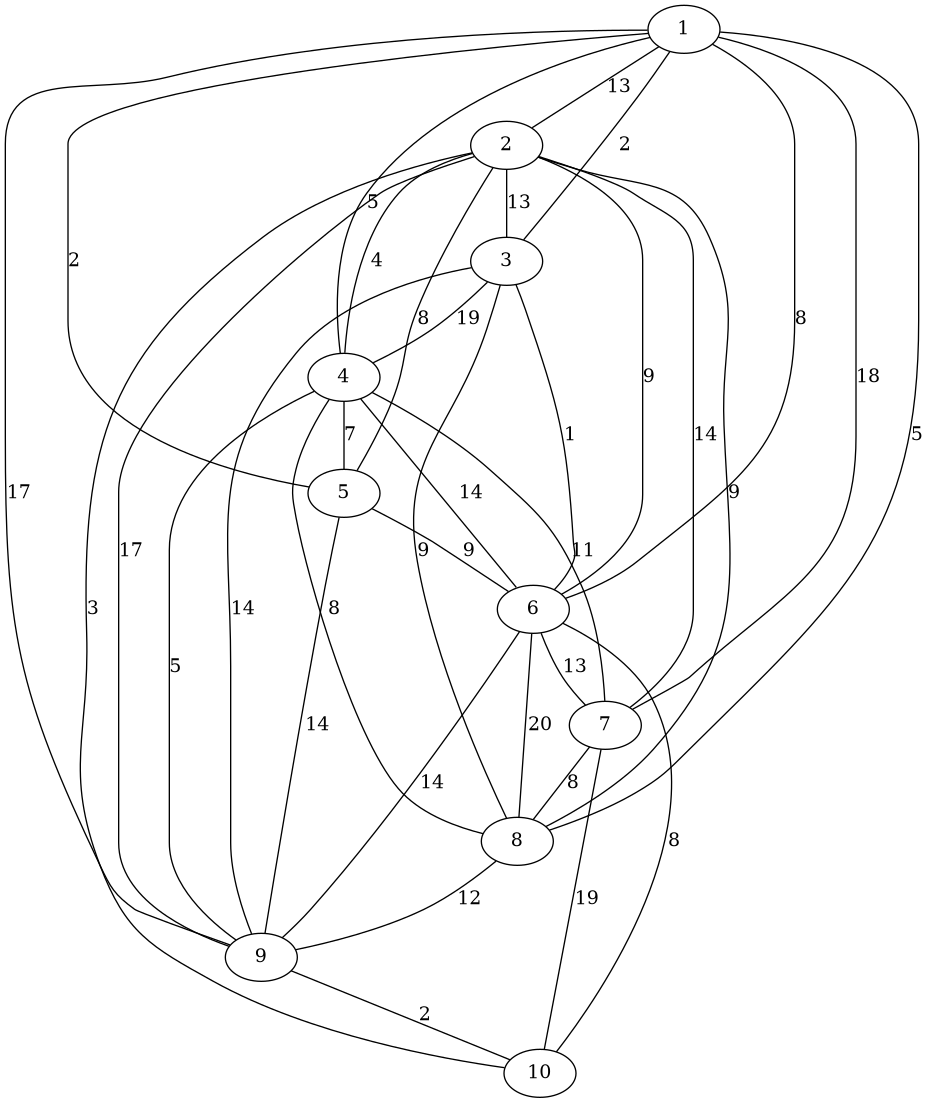
\includegraphics[width=300pt]{graph_size_10_4.png}
		\caption{Граф 4 с 10 вершинами.}
	\end{figure}
	\begin{figure}[h]
		\centering
		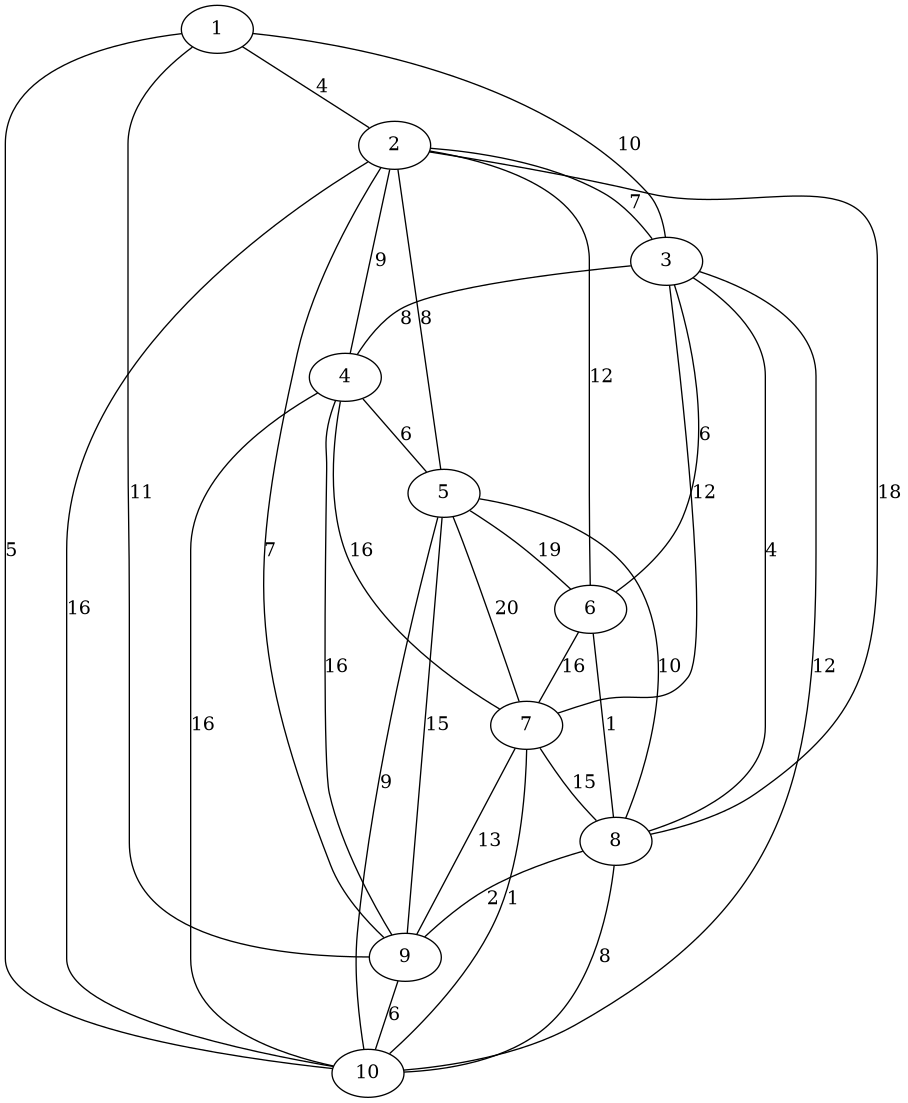
\includegraphics[width=300pt]{graph_size_10_5.png}
		\caption{Граф 5 с 10 вершинами.}
	\end{figure} 

	\begin{figure}[h]
		\centering
		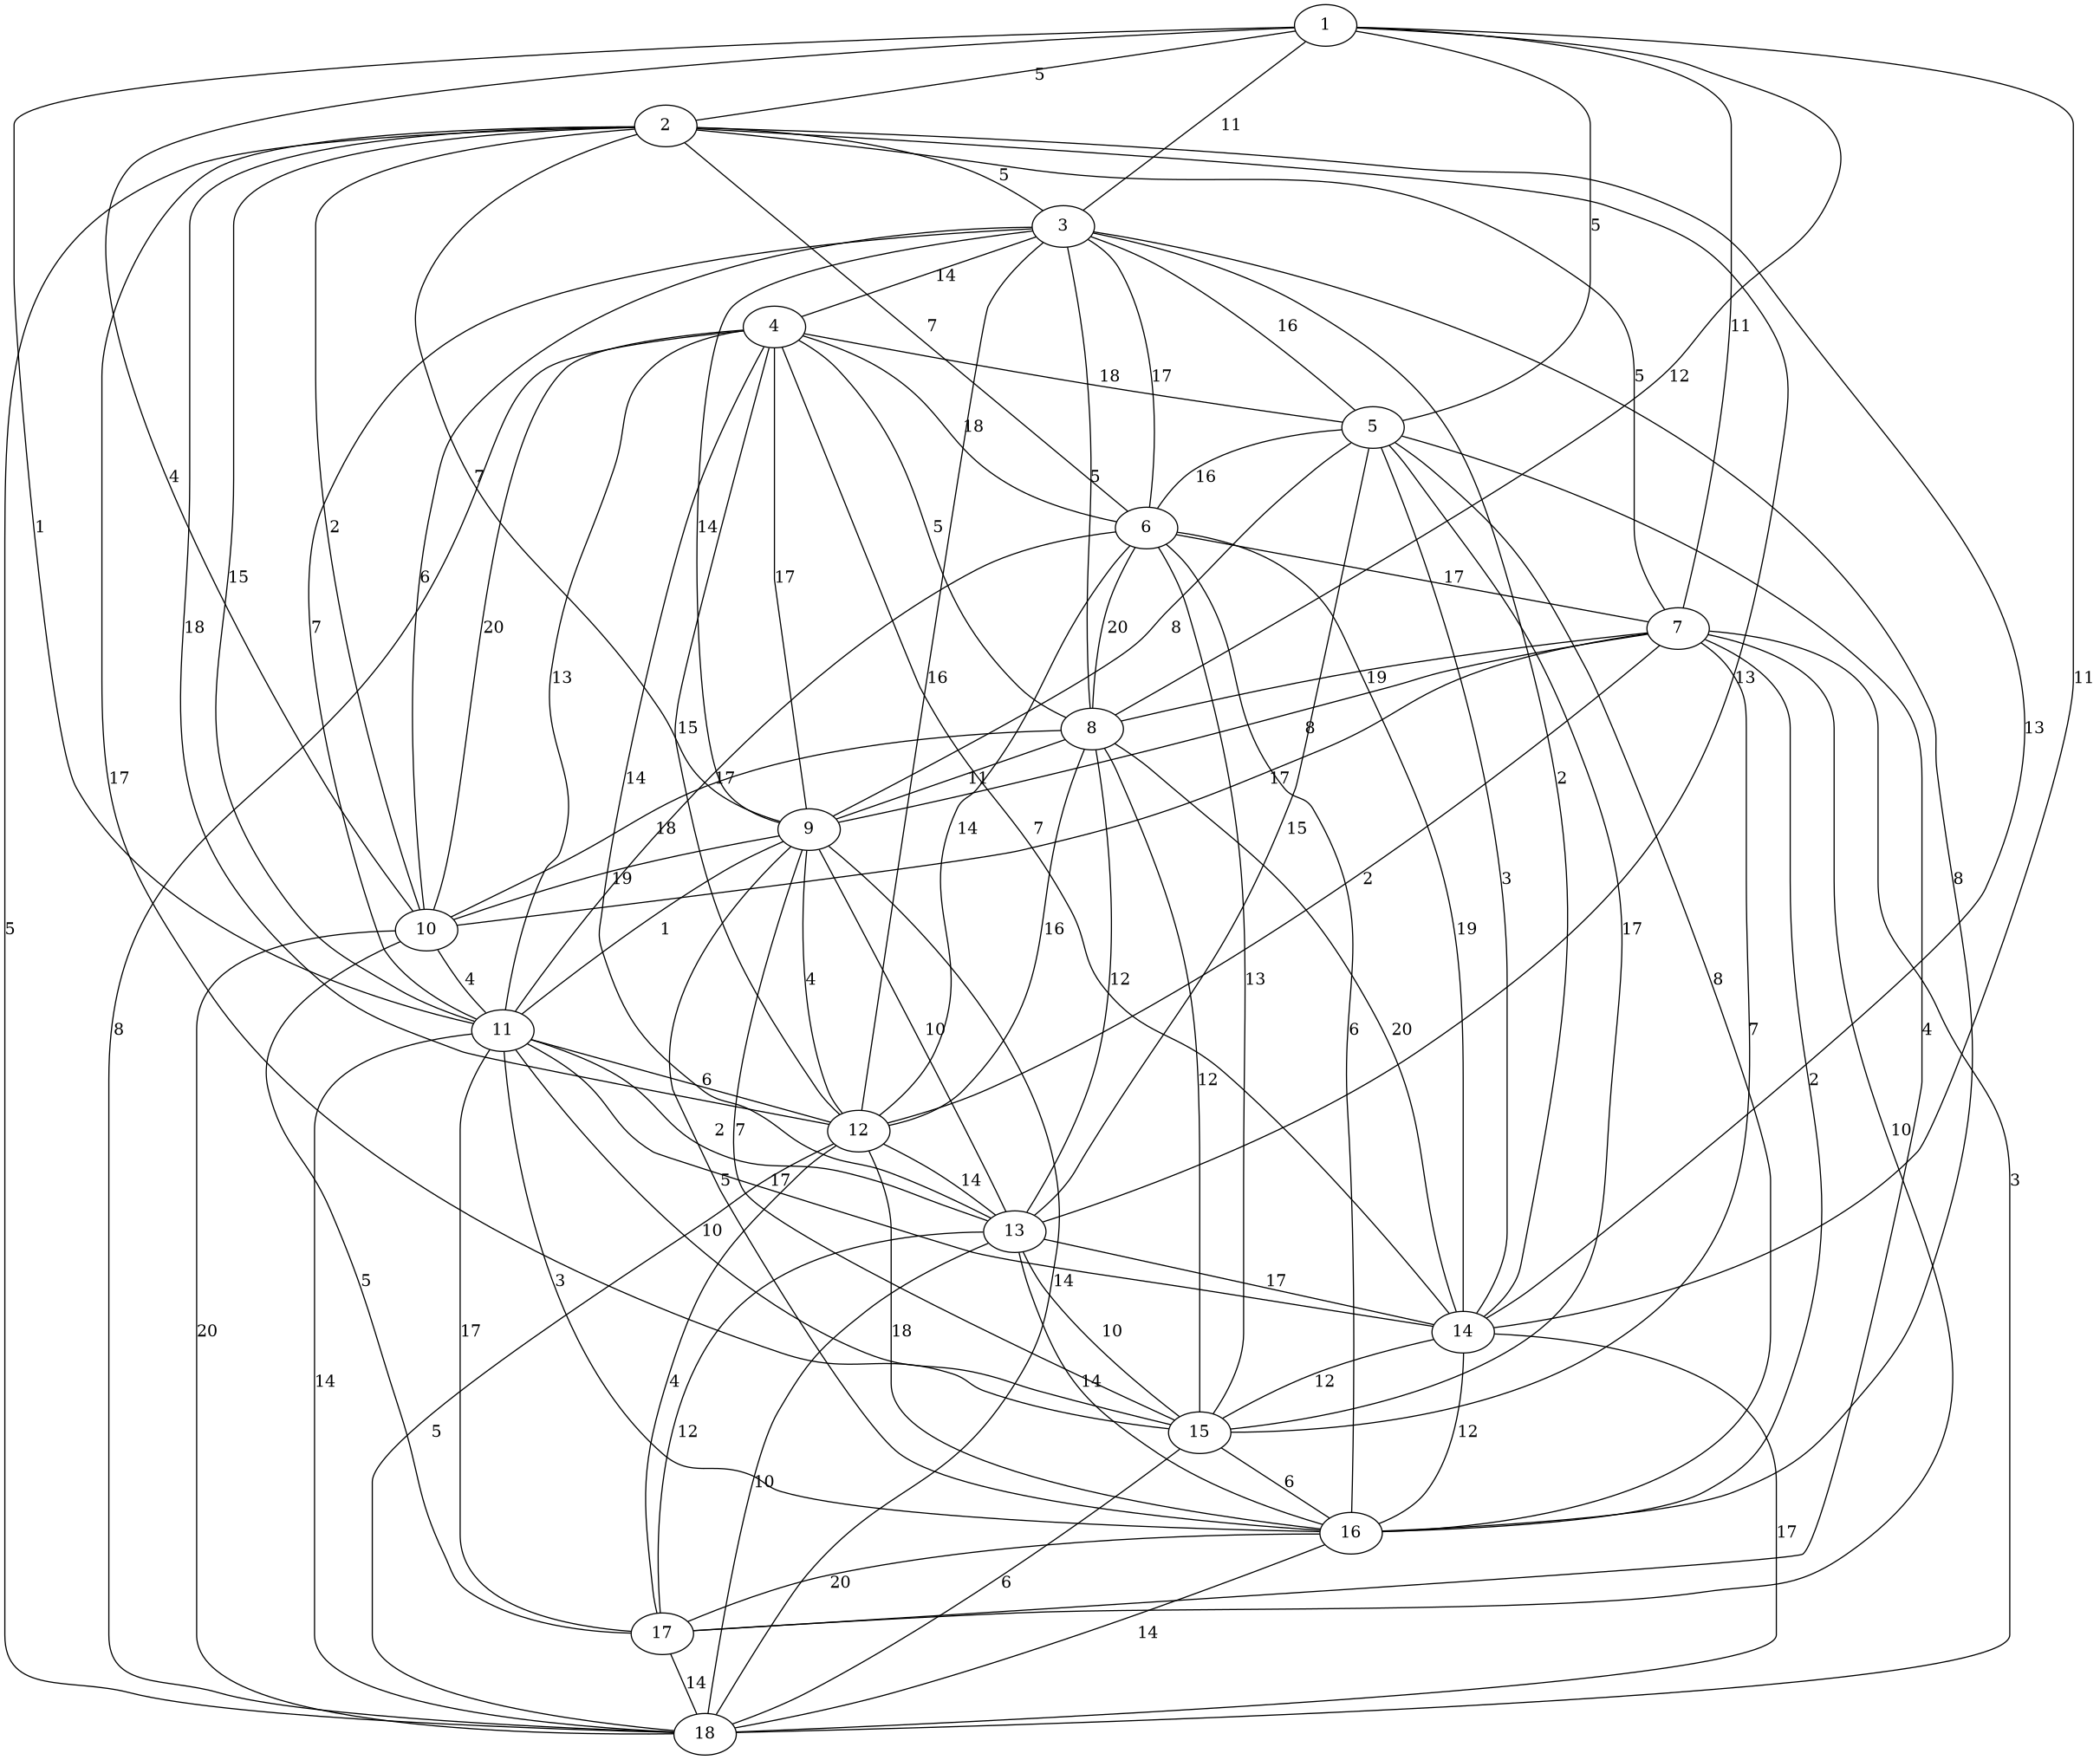
\includegraphics[width=300pt]{graph_size_18_1.png}
		\caption{Граф 1 с 18 вершинами.}
	\end{figure}
	\begin{figure}[h]
		\centering
		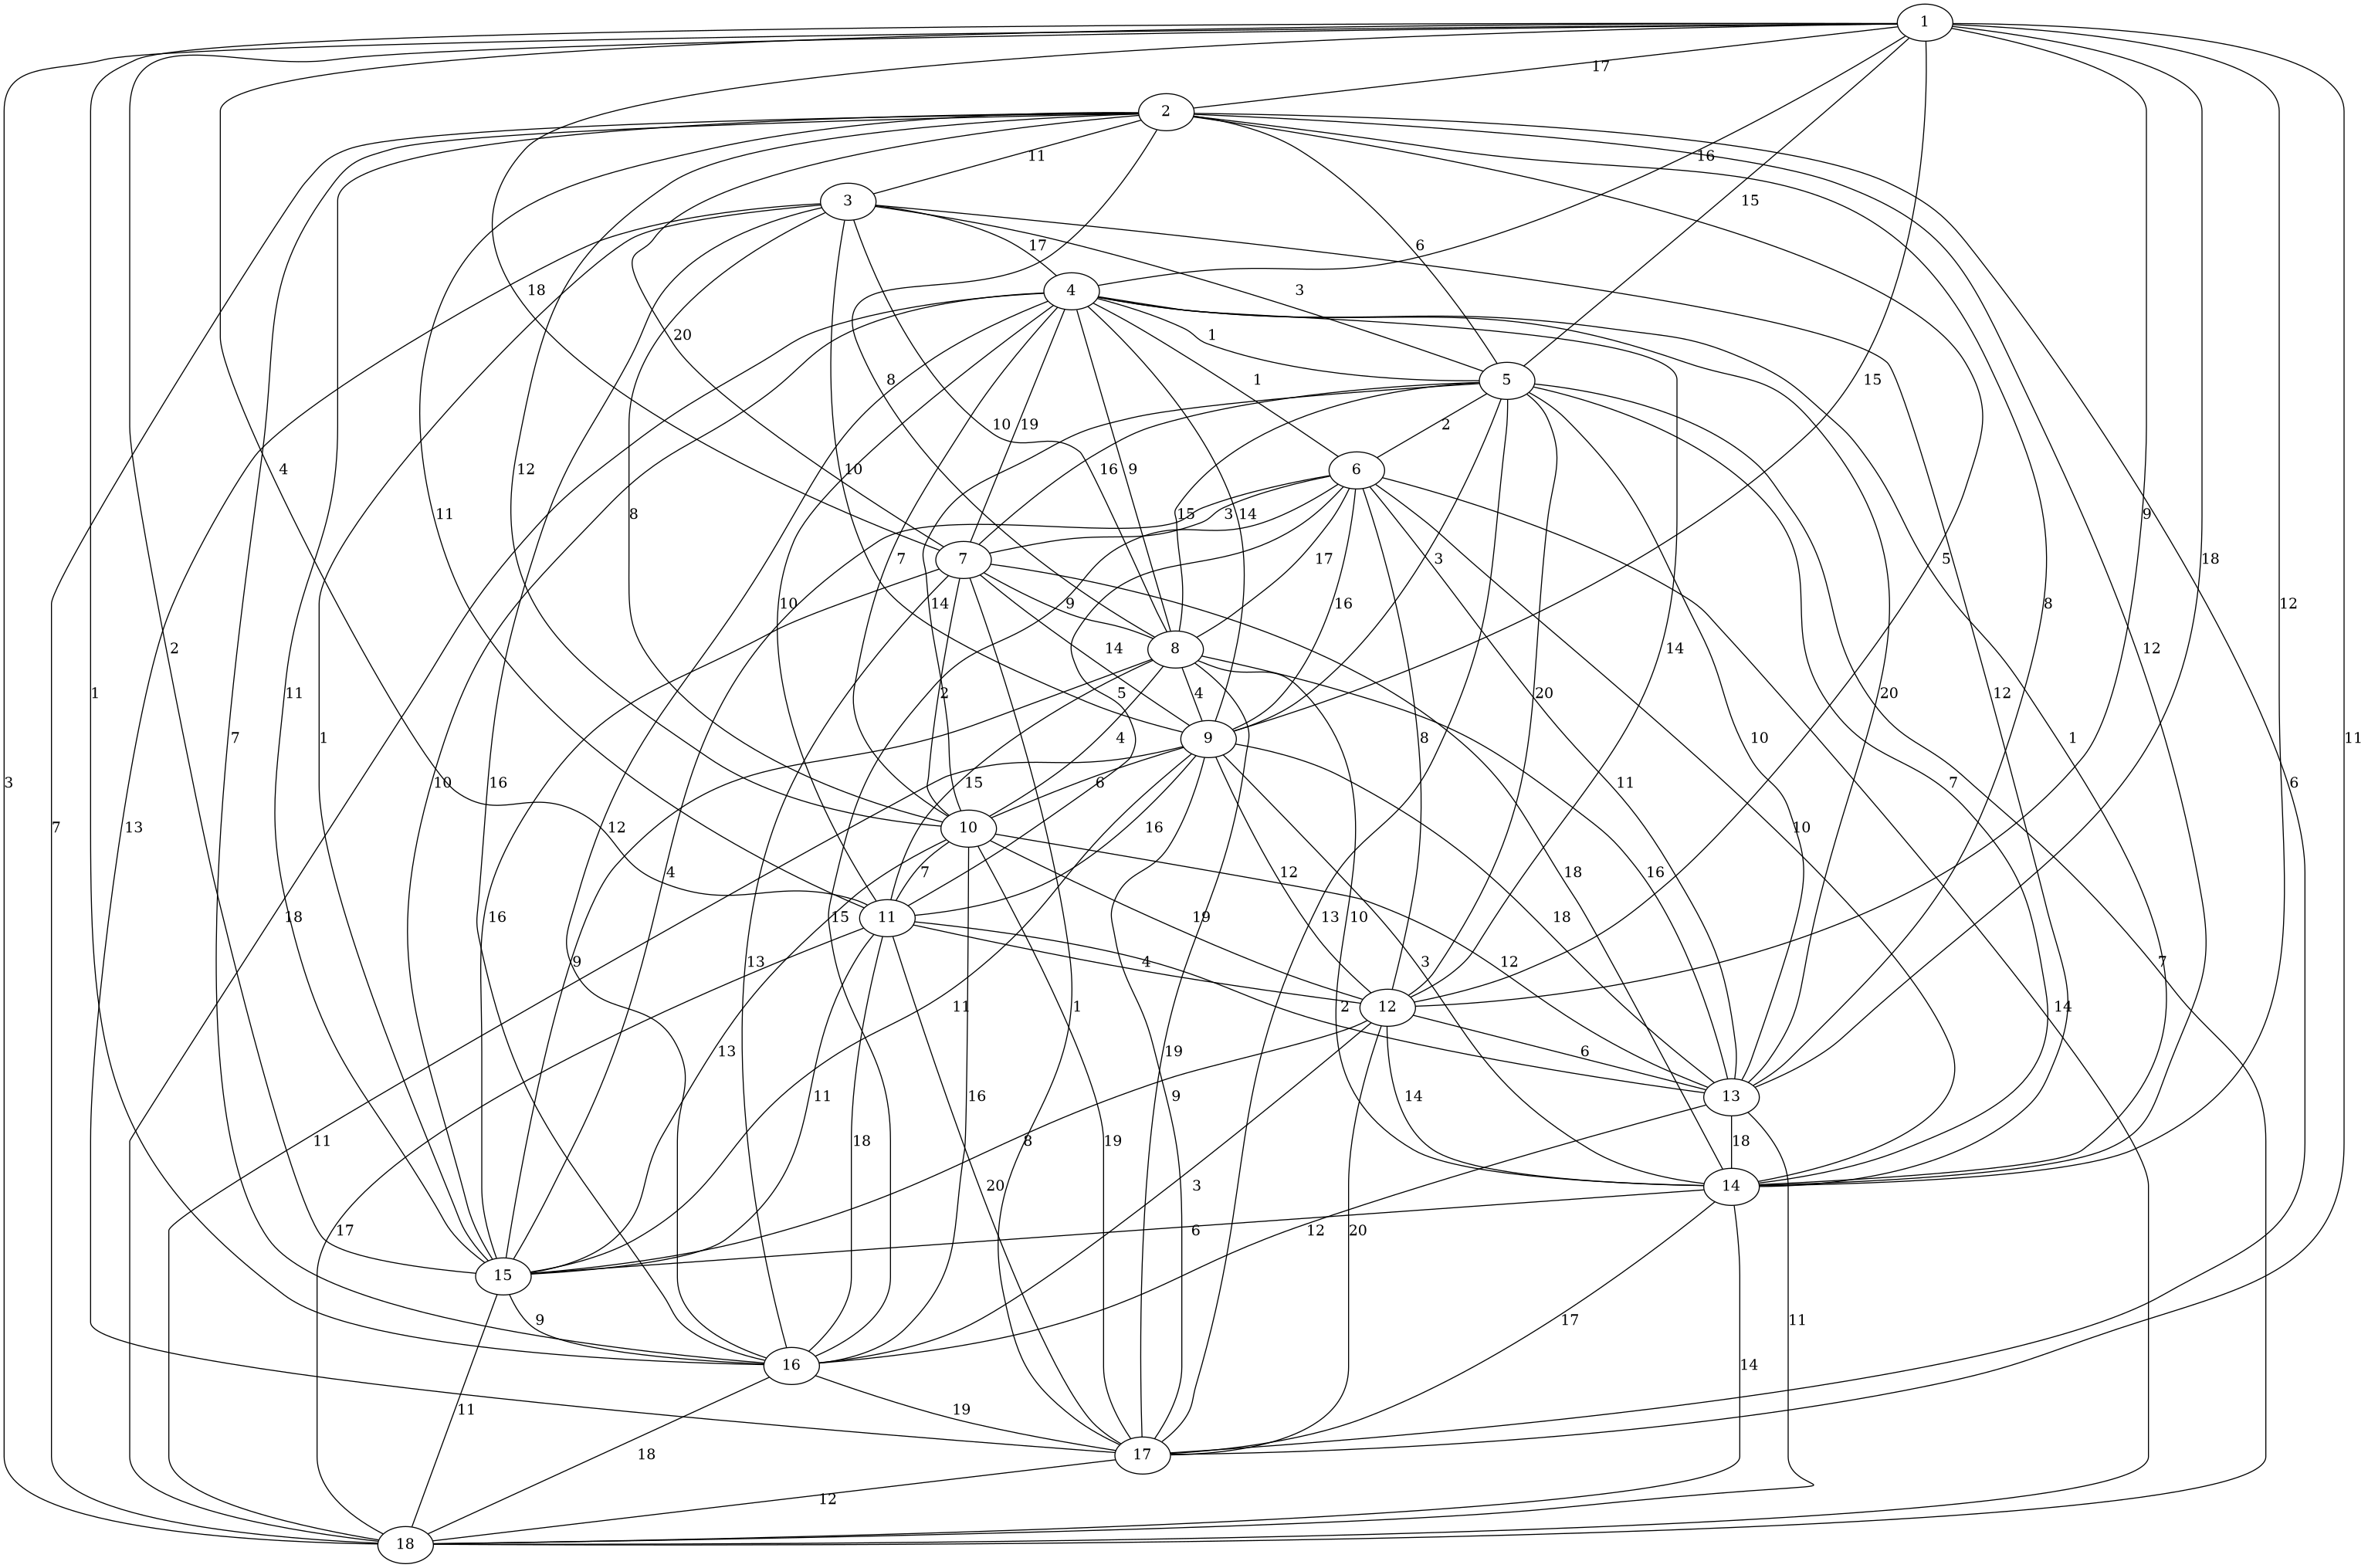
\includegraphics[width=300pt]{graph_size_18_2.png}
		\caption{Граф 2 с 18 вершинами.}
	\end{figure}
	\begin{figure}[h]
		\centering
		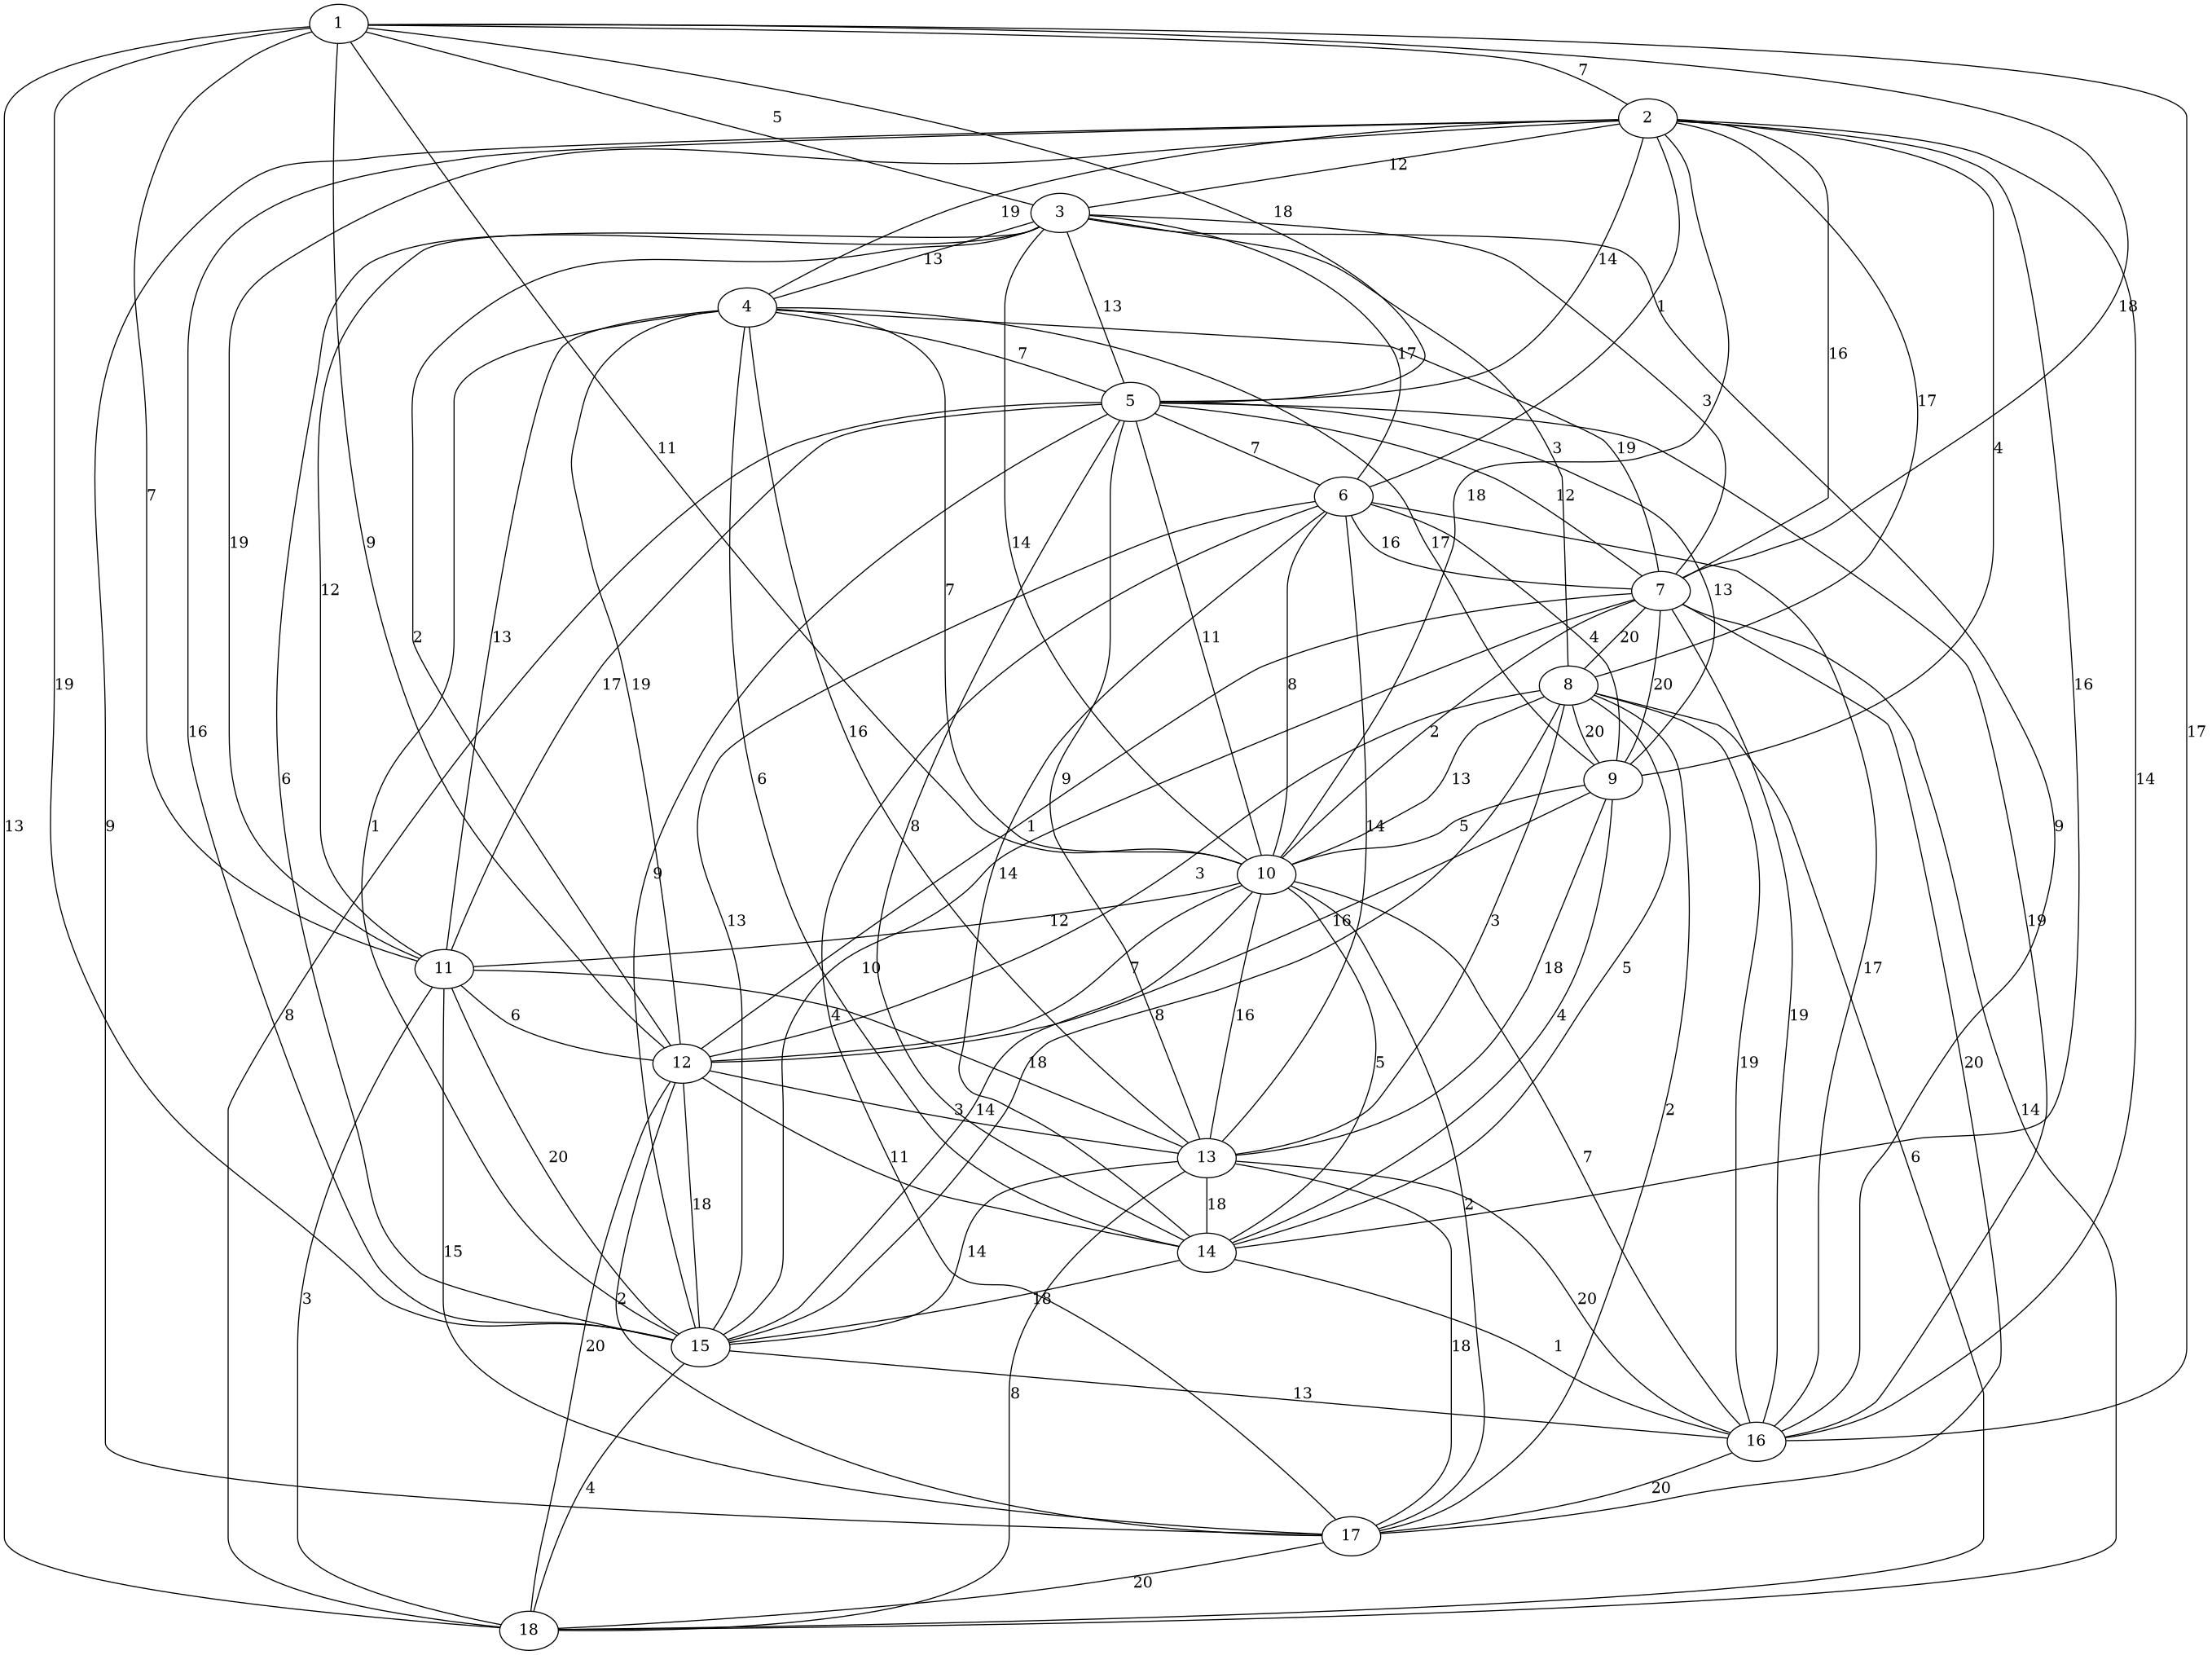
\includegraphics[width=300pt]{graph_size_18_3.png}
		\caption{Граф 3 с 18 вершинами.}
	\end{figure}
	\begin{figure}[h]
		\centering
		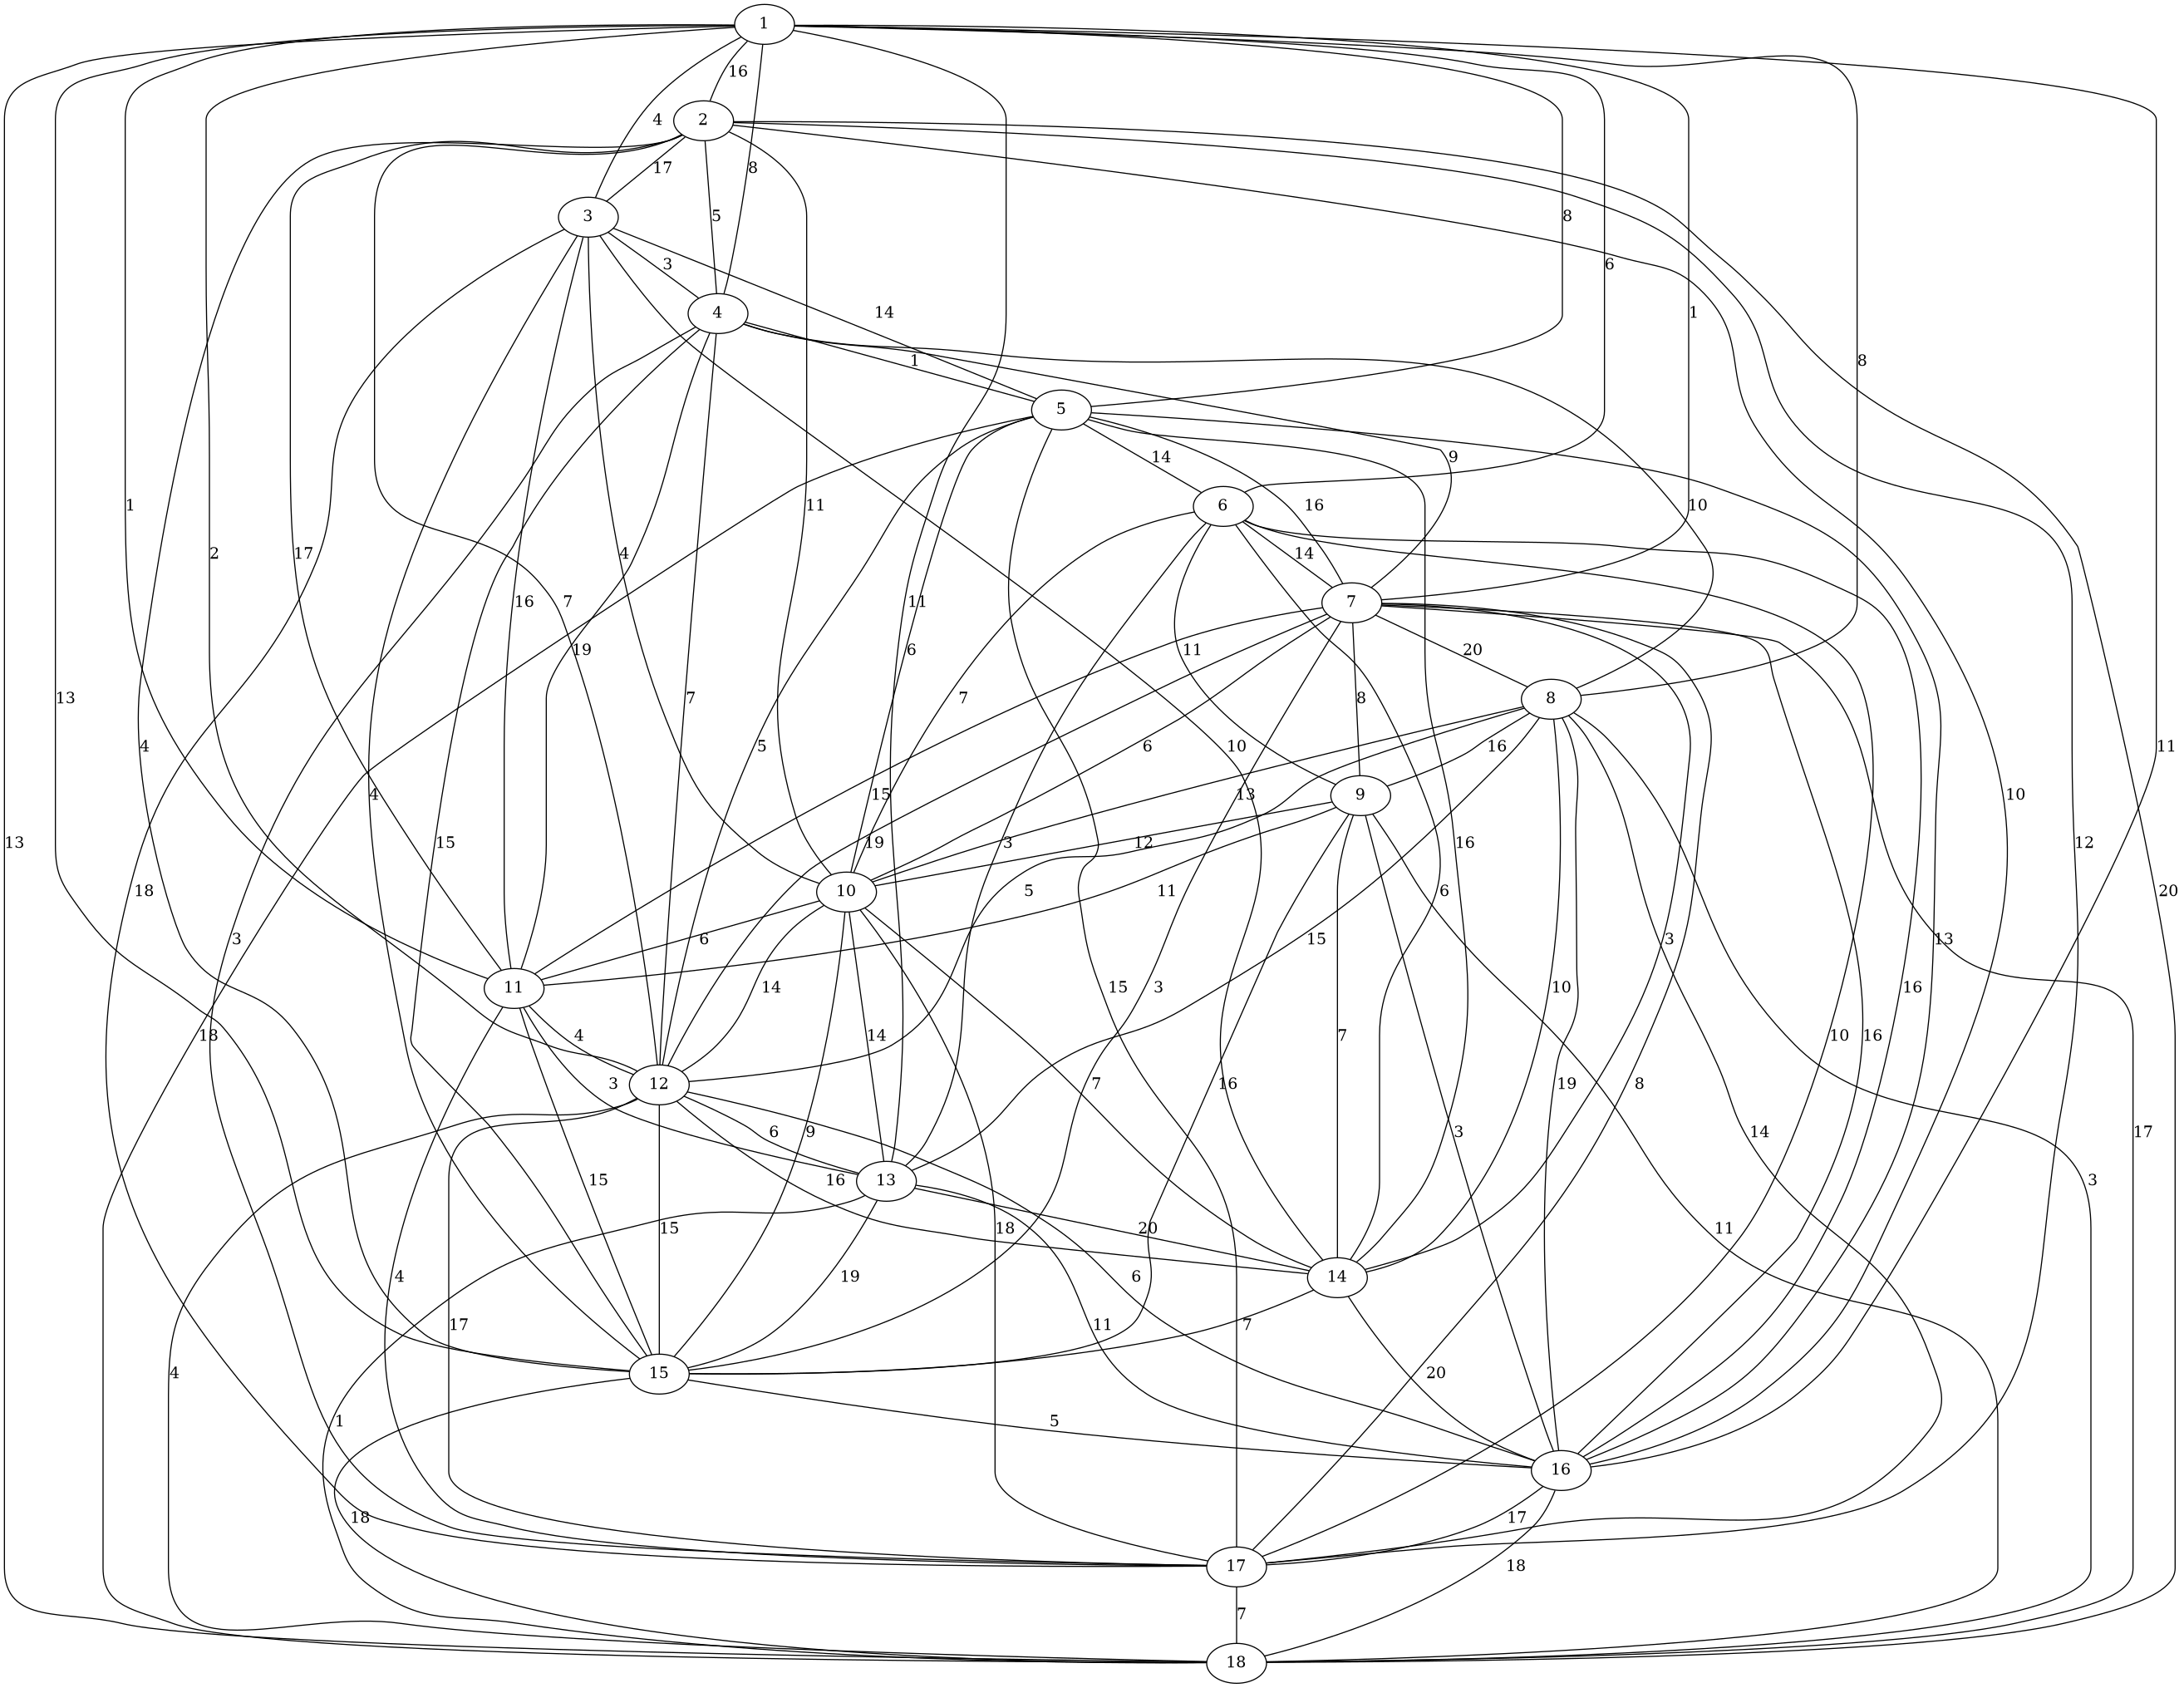
\includegraphics[width=300pt]{graph_size_18_4.png}
		\caption{Граф 4 с 18 вершинами.}
	\end{figure}
	\begin{figure}[h]
		\centering
		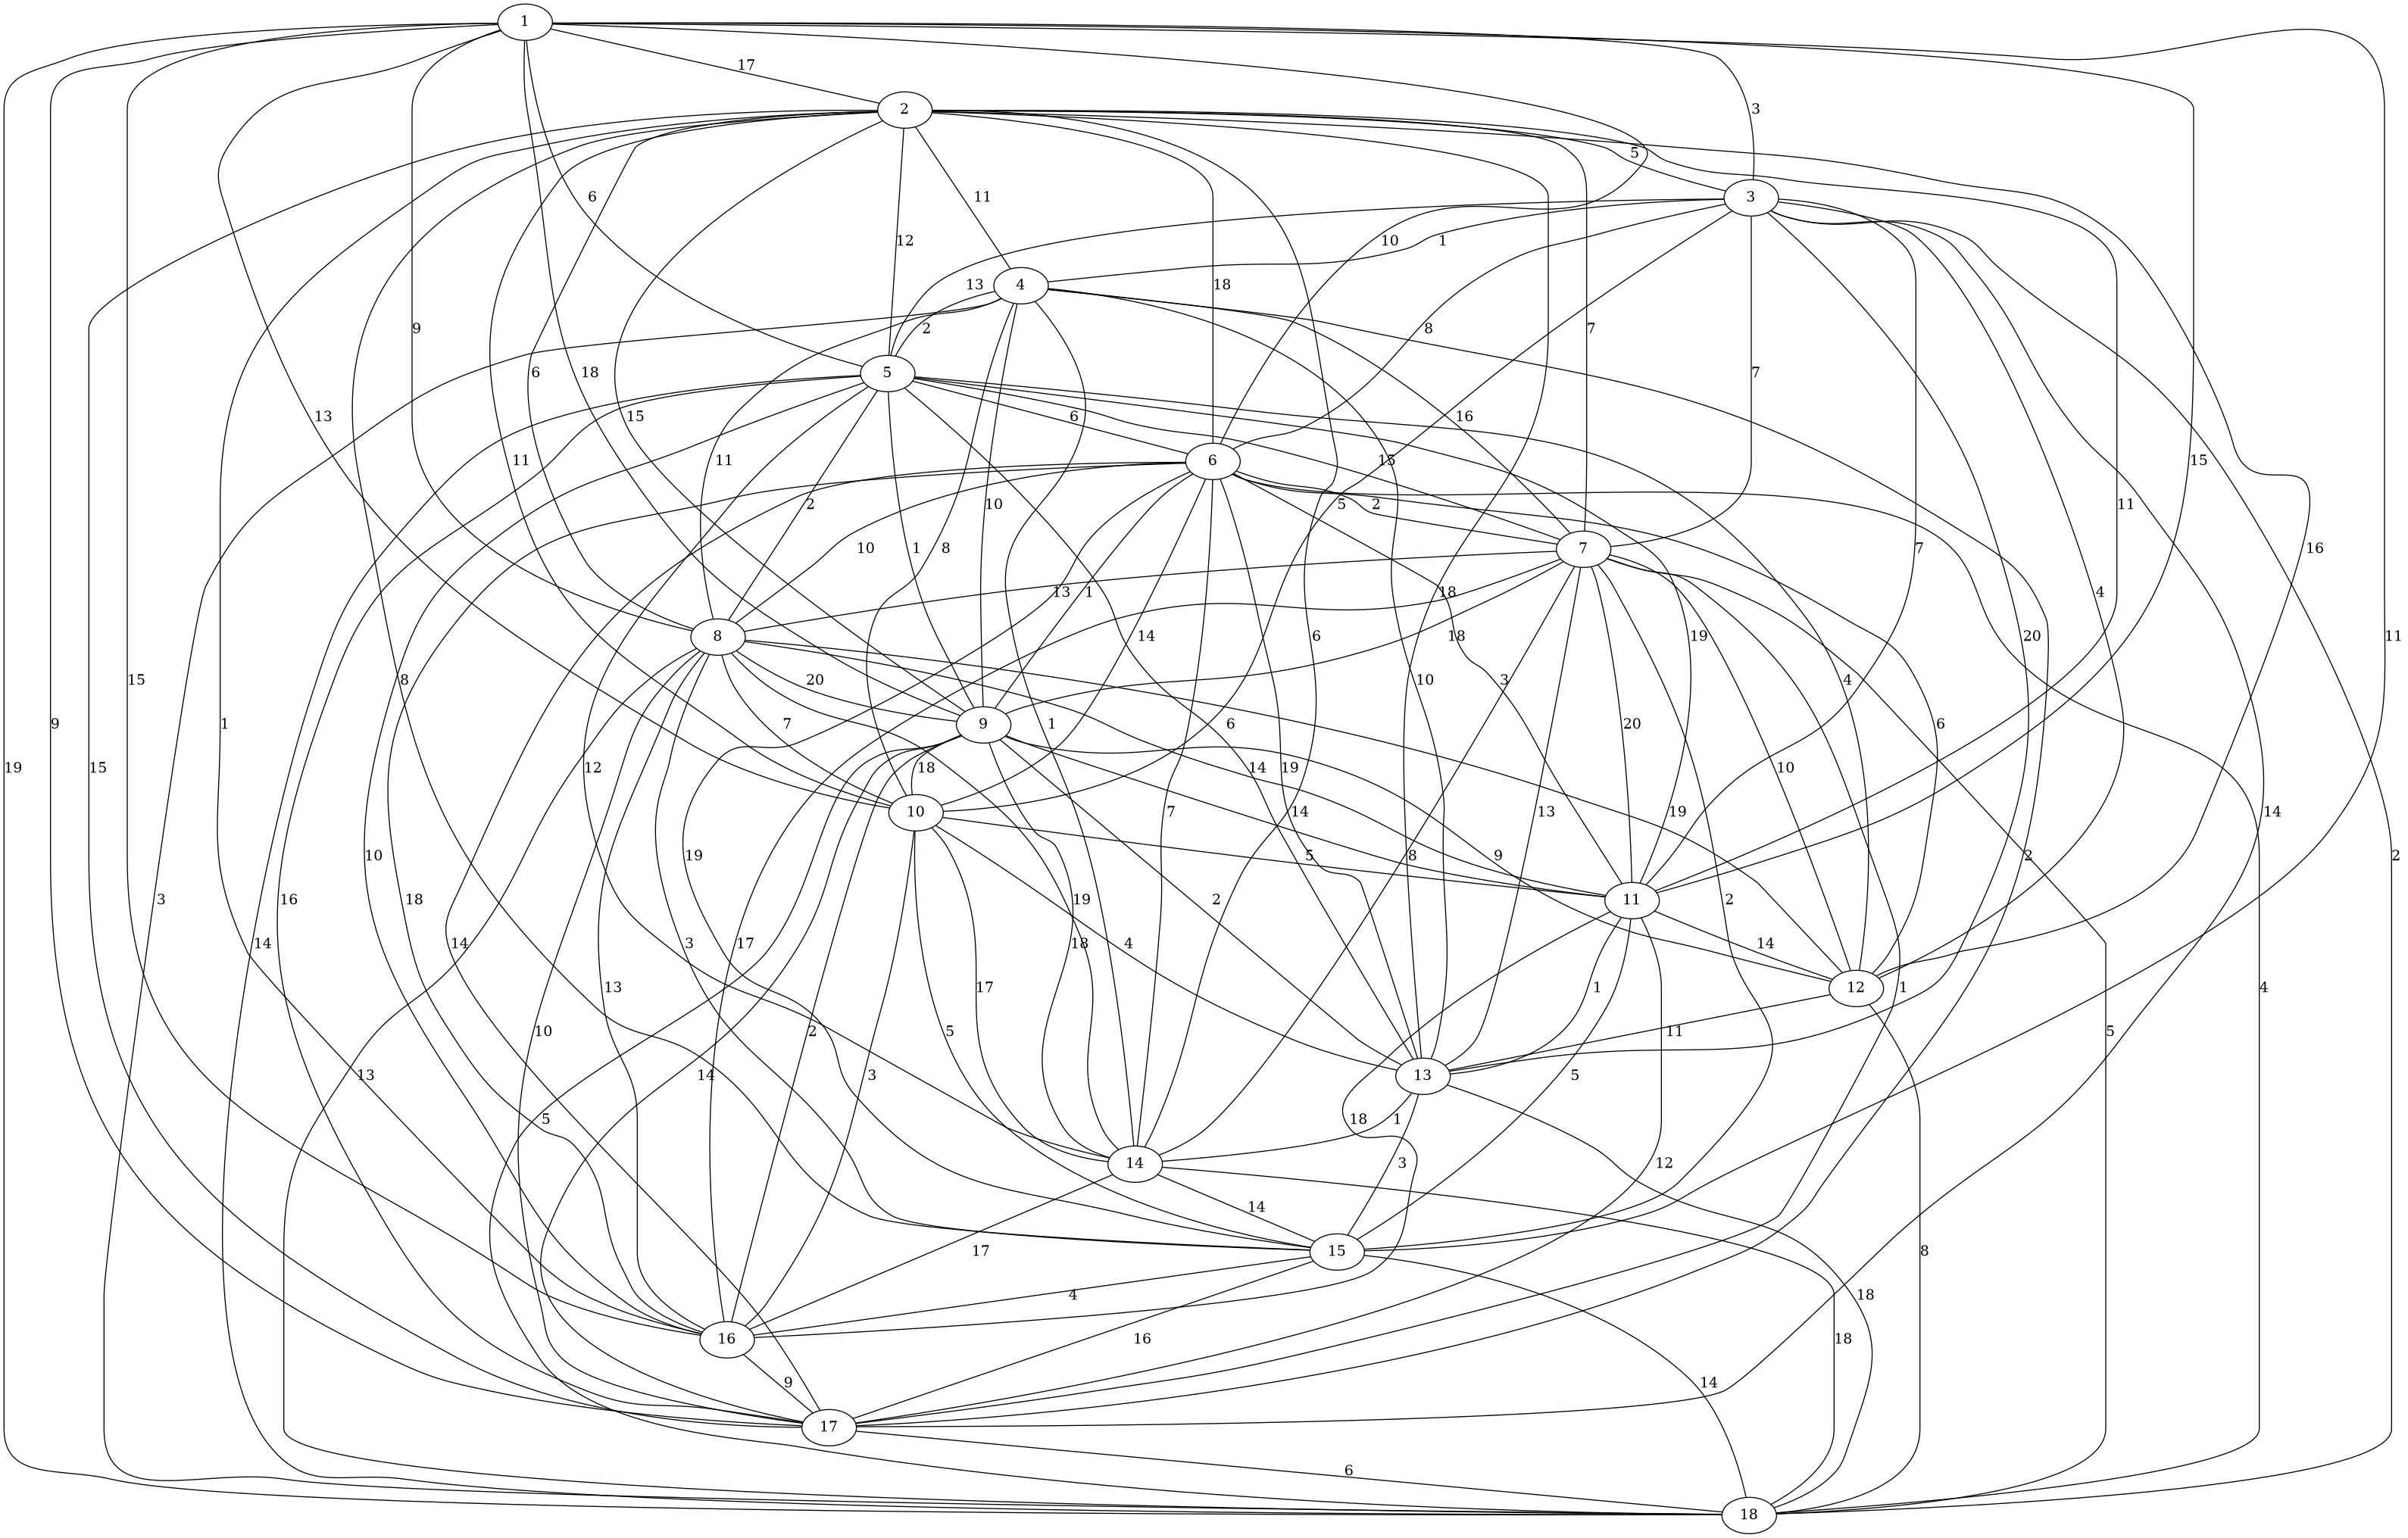
\includegraphics[width=300pt]{graph_size_18_5.png}
		\caption{Граф 5 с 18 вершинами.}
	\end{figure} 

	\begin{figure}[h]
		\centering
		\includegraphics[width=300pt]{graph_size_27_1.png}
		\caption{Граф 1 с 27 вершинами.}
	\end{figure}
	\begin{figure}[h]
		\centering
		\includegraphics[width=300pt]{graph_size_27_2.png}
		\caption{Граф 2 с 27 вершинами.}
	\end{figure}
	\begin{figure}[h]
		\centering
		\includegraphics[width=300pt]{graph_size_27_3.png}
		\caption{Граф 3 с 27 вершинами.}
	\end{figure}
	\begin{figure}[h]
		\centering
		\includegraphics[width=300pt]{graph_size_27_4.png}
		\caption{Граф 4 с 27 вершинами.}
	\end{figure}
	\begin{figure}[h]
		\centering
		\includegraphics[width=300pt]{graph_size_27_5.png}
		\caption{Граф 5 с 27 вершинами.}
	\end{figure} 

	\begin{figure}[h]
		\centering
		\includegraphics[width=300pt]{graph_size_35_1.png}
		\caption{Граф 1 с 35 вершинами.}
	\end{figure}
	\begin{figure}[h]
		\centering
		\includegraphics[w35th=300pt]{graph_size_35_2.png}
		\caption{Граф 2 с 35 вершинами.}
	\end{figure}
	\begin{figure}[h]
		\centering
		\includegraphics[w35th=300pt]{graph_size_35_3.png}
		\caption{Граф 3 с 35 вершинами.}
	\end{figure}
	\begin{figure}[h]
		\centering
		\includegraphics[w35th=300pt]{graph_size_35_4.png}
		\caption{Граф 4 с 35 вершинами.}
	\end{figure}
	\begin{figure}[h]
		\centering
		\includegraphics[width=300pt]{graph_size_27_5.png}
		\caption{Граф 5 с 35 вершинами.}
	\end{figure} 

	\vfill
	\clearpage

	\section*{Выводы}
	\addcontentsline{toc}{section}{Выводы}

\end{document}
